%%%%%%%%%%%%%%%%%%%%%%%%%%%%%%%%%%%%%%%%%%%%%%%%%%%%%%%%%%%%%%%%%%%%%%%%%
% This file is part of the LaTeX sources of the OMDoc 1.2 specifiation
% Copyright (c) 2006 Michael Kohlhase
% This work is licensed by the Creative Commons Share-Alike license
% see http://creativecommons.org/licenses/by-sa/2.5/ for details
\svnInfo $Id: elalg.tex 8481 2009-08-11 05:41:59Z kohlhase $
\svnKeyword $HeadURL: https://svn.omdoc.org/repos/omdoc/branches/omdoc-1.2/doc/spec/elalg.tex $
%%%%%%%%%%%%%%%%%%%%%%%%%%%%%%%%%%%%%%%%%%%%%%%%%%%%%%%%%%%%%%%%%%%%%%%%%

\begin{tchapter}[id=dg-elal]{A Development Graph for Elementary Algebra}
  We will now use the technique presented in the last chapter for the elementary algebraic
  hierarchy. {\Myfigref{rings-dg}} gives an overview of the situation. We will build up
  theories for semigroups, monoids, groups, and rings and a set of theory inclusions from
  these theories to themselves given by the converse of the operation.

\begin{myfig}{rings-dg}{A Development Graph for Elementary Algebra}
\fbox{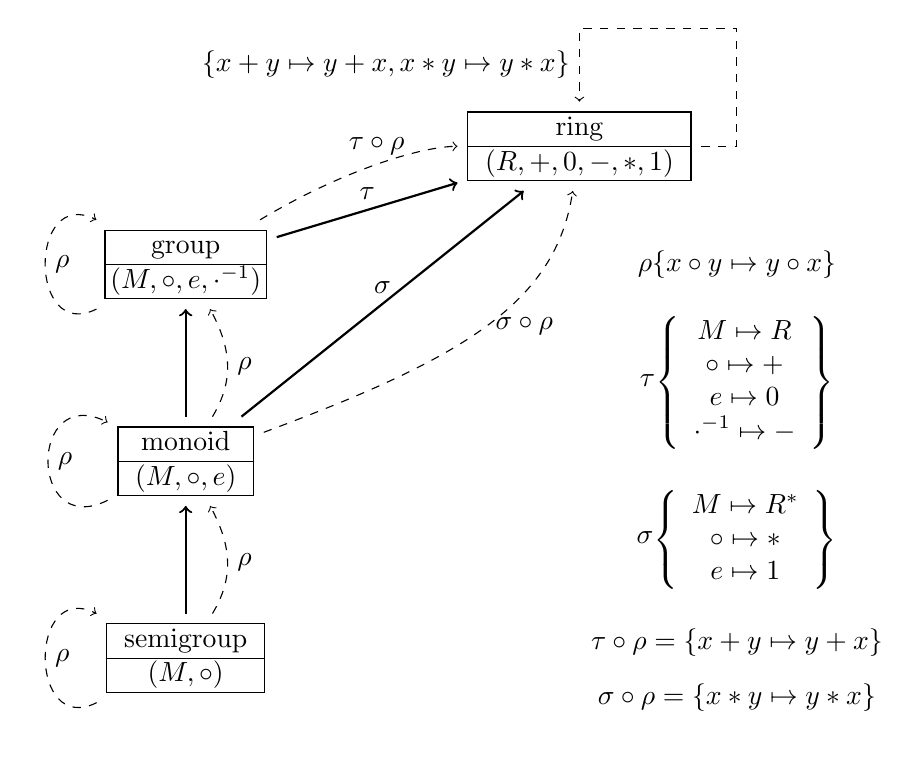
\begin{tikzpicture}
\node (sg) at (1,1)
   {\begin{tabular}{|c|}\hline 
       semigroup\\\hline 
       $(M,\circ)$\\\hline 
     \end{tabular}};
\node (mon) at (1,3.5)
    {\begin{tabular}{|c|}\hline 
      monoid\\\hline
      $(M,\circ,e)$\\\hline
    \end{tabular}};
\node (grp) at (1,6)
    {\begin{tabular}{|c|}\hline 
      group\\\hline
      \kern-1ex$(M,\circ,e,\cdot^{-1})\kern-1ex$\\\hline
    \end{tabular}};

\node (ring) at (6,7.5)
    {\begin{tabular}{|c|}\hline 
      ring\\\hline
      $(R,+,0,-,*,1)$\\\hline
    \end{tabular}};
\node (sigma) at (8,2.5)
    {$\sigma\deq\scriptscriptstyle\left\{\begin{array}{c}
      M\mapsto R^*\\\circ\mapsto *\\e\mapsto 1
    \end{array}\right\}$};
\node (tau) at (8,4.5)
    {$\tau\deq\scriptscriptstyle\left\{\begin{array}{c}
      M\mapsto R\\\circ\mapsto +\\e\mapsto 0\\\cdot^{-1}\mapsto -
    \end{array}\right\}$};

 \node (ts) at (8,6){$\rho\deq\{x\circ y\mapsto y\circ x\}$};
 \node (sr) at (8,.5){$\sigma\circ\rho=\{x*y\mapsto y*x\}$};
 \node (tr) at (8,1.2){$\tau\circ\rho=\{x+y\mapsto y+x\}$};
 \draw [->,thick](sg) -- (mon);
 \draw [->,thick](mon) -- (grp);
 \draw [->,thick](mon) -- node[above]{$\sigma$} (ring);
 \draw [->,thick](grp) -- node[above]{$\tau$} (ring);p
 \draw [->,dashed](mon) .. controls (4.5,4.8) and (5.7,5.5) .. 
     node[right]{$\sigma\circ\rho$} (ring);
 \draw [->,dashed](grp) .. controls (3,7.2) and (4,7.5) .. 
     node[above]{$\tau\circ\rho$} (ring);
 \draw [->,dashed] (sg) .. controls (-1,0) and (-1,2) .. 
     node[right]{$\rho$}(sg);
 \draw [->,dashed] (mon) .. controls (-1,2.5) and (-1,4.5) .. 
     node[right]{$\rho$}(mon);
 \draw [->,dashed] (grp) .. controls (-1,5) and (-1,7) .. 
     node[right]{$\rho$}(grp);
 \draw [->,dashed] (sg) .. controls (1.6,2) and (1.6,2.4) .. 
     node[right]{$\rho$}(mon);
 \draw [->,dashed] (mon) .. controls (1.6,4.5) and (1.6,4.9) .. 
     node[right]{$\rho$}(grp);
 \draw [->,dashed] (ring) -- (8,7.5) -- (8,9) -- (6,9) --
     node[left]{$\{x+y\mapsto y+x,x*y\mapsto y*x\}$} (ring);
\end{tikzpicture}}
\end{myfig}

We start off with the theory for {\emin{semigroup}s}. It introduces two symbols, the base
set $M$ and the operation $\circ$ on $M$ together with two axioms that state that $M$ is
closed under $\circ$ and that $\circ$ is associative on $M$. We have a structural theory
inclusion from this theory to itself that uses the fact that $M$ together with the
converse $\sigma(\circ)$ of $\circ$ is also a semigroup: the obligation for the axioms can
be justified by themselves (for the closure axiom we have
$\sigma(\allcdot{x,y\in{M}}{x\circ y\in{M}})=\allcdot{y,x\in{M}}{x\circ y\in{M}}$, which
is logically equivalent to the axiom.)

\begin{lstlisting}[mathescape,
  index={theory-inclusion,morphism,requation}]
<theory xml:id="semigroup">
  <symbol name="base-set"/>
  <presentation for="#base-set"><use format="default">$M$</use></presentation>
  <symbol name="op"/>
  <presentation for="#op"><use format="default">$\circ$</use></presentation>
  <axiom xml:id="closed.ax"><FMP>$\allcdot{x,y\in{M}}{x\circ y\in{M}}$</FMP></axiom>
  <axiom xml:id="assoc.ax">
    <FMP>$\allcdot{x,y,z\in{M}}{(x\circ y)\circ z=x\circ(y\circ z)}$</FMP>
  </axiom>
</theory>

<theory-inclusion xml:id="sg-conv-sg" from="#semigroup" to="#semigroup">
  <morphism xml:id="sg-conv-sg.morphism">
    <requation>$X\circ Y\leadsto Y\circ X$</requation>
  </morphism>
  <obligation assertion="conv.closed" induced-by="#closed.ax"/>
  <obligation assertion="#assoc.ax" induced-by="#assoc.ax"/>
</theory-inclusion>
\end{lstlisting}
The theory of {\emin{monoid}s} is constructed as an extension of the theory of semigroups
with the additional unit axiom, which states that there is an element that acts as a
(right) unit for $\circ$. As always, we state that there is a unique such unit, which
allows us to define a new symbol $e$ using the
{\atwintoo{definite}{description}{operator}} $\thatcdot{x}{}$: If there is a unique $x$,
such that $\bA$ is true, then the construction $\thatcdot{x}\bA$ evaluates to $x$, and is
undefined otherwise. We also prove that this $e$ also acts as a left unit for $\circ$.

\begin{erratum}[reported-by=Michael Kohlhase,date=2009-08-11]{{\texttt{for}} attribute on
    {\texttt{definition}} should be of type {\texttt{NCNames}}}
\begin{lstlisting}[mathescape]
<theory xml:id="monoid">
  <imports xml:id="sg2mon" from="#semigroup"/>
  <axiom xml:id="unit.ax"><FMP>$\excdot{x\in{M}}{\allcdot{y\in{M}}{y\circ x=y}}$</FMP></axiom>
  <assertion xml:id="unit.unique"><FMP>$\exucdot{x\in{M}}{\allcdot{y\in{M}}{y\circ x=y}}$</FMP></assertion>
  <symbol name="unit" xml:id=''unit''/>
  <presentation for="#unit"><use format="default">e</use></presentation>
  <definition xml:id="unit.def" for="unit" type="simple" existence="#unit.unique">
    $\thatcdot{x\in{M}}{\allcdot{y\in{M}}{y\circ x=y}}$
  </definition>
  <assertion xml:id="left.unit"><FMP>$\allcdot{x\in{M}}{e\circ x=x}$</FMP></assertion>
  <symbol name="setstar" xml:id=''setstar''/>
  <presentation for="#setstar" fixity="postfix">
    <use format="default">$^*$</use>
  </presentation>
  <definition xml:id="ss.def" for="setstar" type="implicit">
    $\allcdot{S\subseteq{M}}{S^*=S\backslash\set{e}}$
  </definition>
</theory>
\end{lstlisting}
\end{erratum}
Building on this, we first establish an axiom-selfinclusion from the theory of
monoids to itself. We can make this into a {\twintoo{theory}{selfinclusion}} using
the theory-selfinclusion for semigroups as the local part of a path justification
(recall that theory inclusions are axiom inclusions by construction) and the
definitional theory inclusion induced by the import from semigroups to monoids as
the global path.
\begin{lstlisting}[mathescape,index={axiom-inclusion,theory-inclusion,morphism,obligation}]
<axiom-inclusion  xml:id="mon-conv-mon.local" from="#monoid" to="#monoid">
  <morphism base="#sg-conv-sg.morphism"/>
  <obligation assertion="#left.unit" induced-by="#unit.ax"/>
</axiom-inclusion>

<axiom-inclusion xml:id="sg-conv-mon" from="#semigroup" to="#monoid">
  <morphism base="#sg-conv-sg.morphism"/>
  <path-just local="#sg-conv-sg" globals="#sg2mon"/>
</axiom-inclusion>
<theory-inclusion xml:id="mon-conv-mon.global" from="#monoid" to="#monoid">
  <morphism base="#sg-conv-sg.morphism"/>
  <decomposition links="#sg-conv-sg #sg-conv-mon"/>
</theory-inclusion>
\end{lstlisting}
Note that all of these axiom inclusions have the same morphism (denoted by $\rho$
in {\myfigref{rings-dg}}), in {\omdoc} we can share this structure using the
{\attribute{base}{morphism}} on the {\element{morphism}} element. This normally
points to a morphism that is the base for extension, but if the
{\element{morphism}} element is empty, then this just means that the morphisms are
identical. 

For groups, the situation is very similar: We first build a theory of groups by
adding an axiom claiming the existence of inverses and constructing a new function
$\cdot^{-1}$ from that via a definite description. 

\begin{erratum}[reported-by=Michael Kohlhase,date=2009-08-11]{{\texttt{for}} attribute on
    {\texttt{definition}} should be of type {\texttt{NCNames}}}
\begin{lstlisting}[mathescape]
<theory xml:id="group">
  <imports xml:id="mon2grp" from="#monoid"/>
  <axiom xml:id="inv.ax"><FMP>$\allcdot{x\in{M}}{\excdot{y\in{M}}{x\circ y=e}}$</FMP></axiom>
  <symbol name="inv" xml:id=''inv''/>
  <presentation for="#inv" role="applied">
    <use format="default" lbrack="" rbrack="" fixity="postfix">$^{-1}$</use>
  </presentation>
  <definition xml:id="inv.def" for="inv" type="pattern">
    <requation>$x^{-1}\leadsto\thatcdot{y}x\circ y=e$</value></requation>
  </definition>
  <assertion xml:id="conv.inv"><FMP>$\allcdot{x\in{M}}{\excdot{y\in{M}}{y\circ x=e}}$</FMP></assertion>
</theory>
\end{lstlisting}
\end{erratum}
Again, we have to establish a couple of axiom inclusions to justify the theory
inclusion of interest. Note that we have one more than in the case for monoids,
since we are one level higher in the inheritance structure, also, the local chains
are one element longer.
\begin{lstlisting}[mathescape,index={axiom-inclusion,theory-inclusion}]
<axiom-inclusion xml:id="grp-conv-grp.local" from="#group" to="#group">
  <morphism base="#sg-conv-sg.morphism"/>
  <obligation assertion="conv.inv" induced-by="#inv.ax"/>
</axiom-inclusion>
<axiom-inclusion xml:id="sg-conv-grp" from="#semigroup" to="#group">
  <morphism base="#sg-conv-sg.morphism"/>
  <path-just local="#sg-conv-sg" globals="#mon2grp #sg2mon"/>
</axiom-inclusion>
<axiom-inclusion xml:id="mon-conv-grp" from="#monoid" to="#group">
  <morphism base="#sg-conv-sg.morphism"/>
  <path-just local="#mon-conv-mon.local" globals="#mon2grp"/>
</axiom-inclusion>
<theory-inclusion xml:id="grp-conv-grp" from="#group" to="#group">
  <morphism base="#sg-conv-sg.morphism"/>
  <decomposition links="#sg-conv-grp #mon-conv-grp #grp-conv-grp.local"/>
</theory-inclusion>
\end{lstlisting}
Finally, we extend the whole setup to a theory of rings. Note that we have a dual import
from {\snippet{group}} and {\snippet{monoid}} with different morphisms (they are
represented by $\sigma$ and $\tau$ in {\myfigref{rings-dg}}). These rename all of the
imported symbols apart (interpreting them as additive and multiplicative) except of the
punctuated set constructor $\cdot^*$, which is imported from the additive group structure
only. We avoid a name clash with the operator that would have been imported from the
multiplicative structure by specifying that this is not imported using the
{\attribute{hiding}{morphism}} on the {\element{morphism}} in the respective
{\element{imports}} element\footnote{An alternative (probably better) to this would have
  been to explicitly include the operators in the morphisms, creating new operators for
  them in the theory of {\snippet{rings}}.  But the present construction allows us to
  exemplify the {\attribute{hiding}{morphism}}, which has not been covered in an example
  otherwise.}.
\begin{erratum}[reported-by=Michael Kohlhase,date=2009-08-11]{{\texttt{for}} attribute on
    {\texttt{definition}} should be of type {\texttt{NCNames}}, totally reworked example}
\begin{lstlisting}[mathescape,index={theory,imports}]
<theory xml:id="ring"> 
  <symbol name="R" xml:id=''R''/>
  <presentation for="#R"><use format="default">R</use></presentation>
  <symbol name="zero"/>
  <presentation for="#zero"><use format="default">0</use></presentation>
 <symbol name="plus"/>
 <presentation for="#plus" role="applied">
    <use format="default">+</use>
  </presentation>
 <symbol name="negative"/>
 <presentation for="#negative" role="applied">
    <use format="default">-</use>
  </presentation>
 <symbol name="times"/>
  <presentation for="#times" role="applied">
    <use format="default">*</use>
  </presentation>
  <symbol name="one"/> 
  <presentation for="#one"><use format="default">1</use></presentation>
  <imports xml:id="add.import" from="#group"> 
    <morphism>$M\mapsto R,x\circ y\mapsto x*y, e\mapsto 1,\cdot^{-1}\mapsto -$</morphism> 
  </imports> 
  <imports xml:id="mult.import" from="#monoid"> 
    <morphism hiding="setstar">$M\mapsto M^*,x\circ y\mapsto x*y, e\mapsto 1$</morphism> 
  </imports> 
  <axiom xml:id="dist.ax"><FMP>$x*(y+z)=(x*y)+(x*z)$</FMP></axiom> 
  <assertion xml:id="dist.conv"><FMP>$(z+y)*x=(z*x)+(y*x)$</FMP></assertion>
</theory>
\end{lstlisting}
\end{erratum}
Again, we have to establish some axiom inclusions to justify the
{\twintoo{theory}{selfinclusion}} we are after in the example. Note that in the
rings case, things are more complicated, since we have a dual import in the theory
of {\snippet{rings}}. Let us first establish the additive part. 
 
\begin{lstlisting}[mathescape,index={axiom-inclusion,theory-inclusion}]
<axiom-inclusion xml:id="sg-conv-rg.add" from="#semigroup" to="#ring">
  <morphism base="#sg-conv-sg.morphism #add.import"/>
  <path-just local="#sg-conv-sg" globals="#sg2mon #mon2grp #add.import "/>
</axiom-inclusion>
<axiom-inclusion xml:id="mon-conv-rg.add" from="#monoid" to="#group">
  <morphism base="#sg-conv-sg.morphism #add.import"/>
  <path-just local="#mon-conv-mon.local" globals="#mon2grp #add.import"/>
</axiom-inclusion>
<axiom-inclusion xml:id="grp-conv-rg.add" from="#group" to="#group">
  <morphism base="#sg-conv-sg.morphism #add.import"/>
  <path-just local="#grp-conv-grp.local" globals="#add.import"/>
</axiom-inclusion>
\end{lstlisting}
The multiplicative part is totally analogous, we will elide it to conserve space.
Using both parts, we can finally get to the local axiom self-inclusion and extend
it to the intended theory inclusion justified by the axiom inclusions established
above.
\begin{lstlisting}[mathescape,index={axiom-inclusion,theory-inclusion}]
<axiom-inclusion xml:id="rg-conv-rg.local" from="#ring" to="#ring">
  <morphism xml:id="rg-conv-rg.morphism">$x+y\mapsto y+x,x*y\mapsto y*x$</morphism>
  <obligation assertion="#dist.conv" induced-by="#dist.ax"/>
</axiom-inclusion>  
<theory-inclusion xml:id="rg-conv-rg" from="#ring" to="#ring">
  <morphism base="#rg-conv-rg.morphism"/>
  <decomposition links="#rg-conv-rg.local 
                        #sg-conv-rg.add  #mon-conv-rg.add  #grp-conv-rg.add
                        #sg-conv-rg.mult #mon-conv-rg.mult #grp-conv-rg.mult"/>
</theory-inclusion>  
\end{lstlisting}
This concludes our example. It could be extended to higher constructs in algebra
like fields, magmas, or vector spaces easily enough using the same methods, but
we have seen the key features already.
\end{tchapter}

%%% Local Variables: 
%%% mode: latex
%%% TeX-master: "omdoc"
%%% End: 
 

% LocalWords:  dg elal sg mon grp linewidth arcangle angleA angleB mathescape
% LocalWords:  requation conv def uniq setstar ss selfinclusion lbrack ts
% LocalWords:  rbrack mult dist sr tr FMP globals inv rg
